 
\documentclass[12pt]{article}
 
\usepackage{listings}
\usepackage{color}
\usepackage{graphicx}
\usepackage{float}
\usepackage{pdfpages}
\usepackage{lmodern}			% Usa a fonte Latin Modern			
\usepackage[T1]{fontenc}		% Selecao de codigos de fonte.
\usepackage[utf8]{inputenc}		% Codificacao do documento (conversão automática dos acentos)

\definecolor{mygreen}{rgb}{0,0.6,0}
\definecolor{mygray}{rgb}{0.5,0.5,0.5}
\definecolor{mymauve}{rgb}{0.58,0,0.82}

\lstset{ 
  backgroundcolor=\color{white},
  basicstyle=\ttfamily\tiny,
  breakatwhitespace=false,         
  breaklines=true,                 
  captionpos=b,                    
  commentstyle=\color{mygreen},    
  escapeinside={\%*}{*)},          
  extendedchars=true,              
  frame=single,                    
  keepspaces=true,                 
  keywordstyle=\color{blue},       
  language=Octave,                 
  morekeywords={=,->},            
  numbers=left,                    
  numbersep=5pt,                   
  numberstyle=\tiny\color{mygray}, 
  rulecolor=\color{black},         
  showspaces=false,                
  showstringspaces=false,          
  showtabs=false,                  
  stepnumber=2,                    
  stringstyle=\color{mymauve},     
  tabsize=2,                       
  title=\lstname
}


\begin{document}

\lstinputlisting[title=WIRTH]{../WIRTH.txt}

\lstinputlisting[title=AFD PROGRAM]{../output/PROGRAM.mdfa}

\begin{figure}[H]
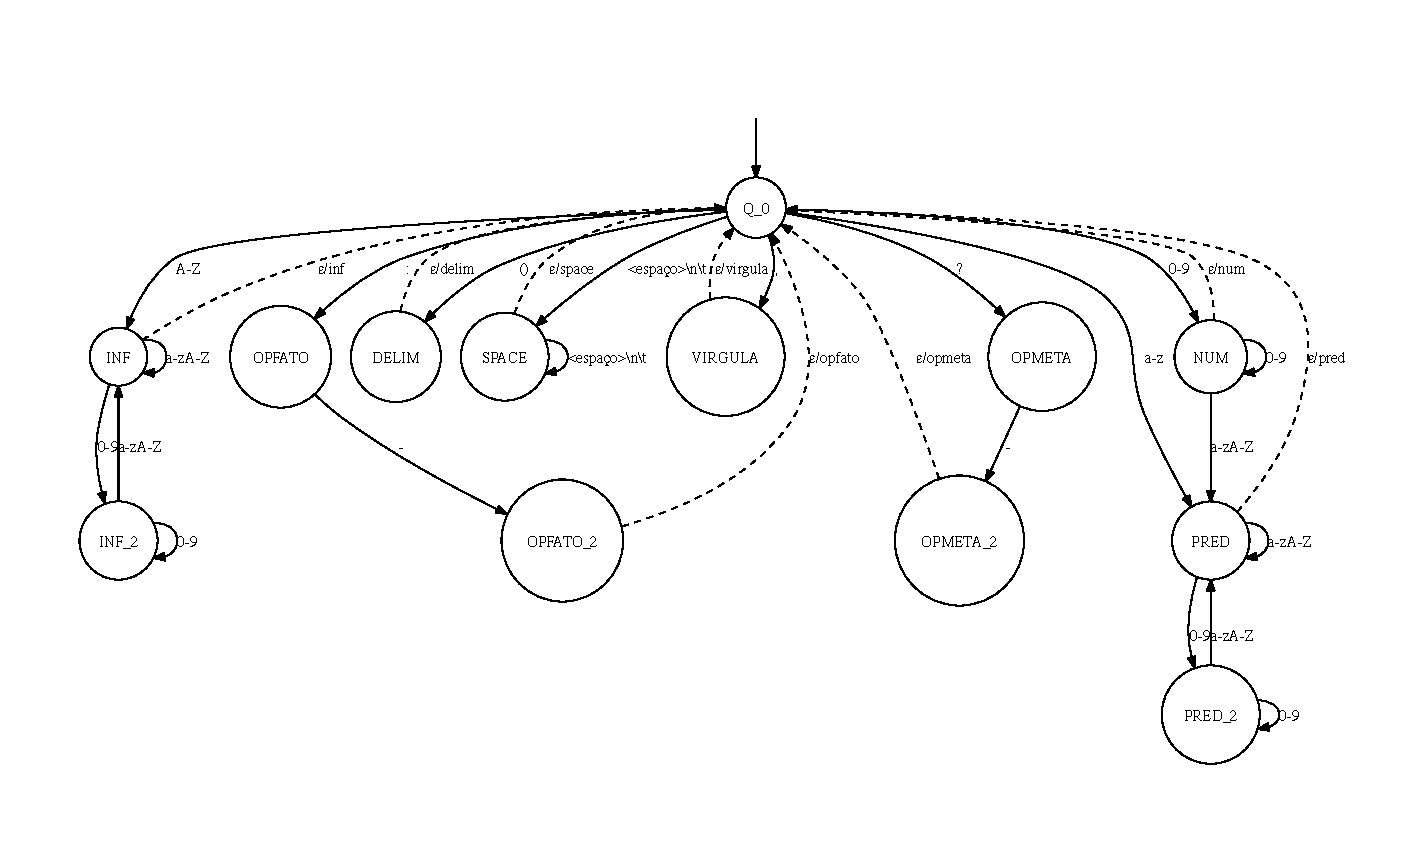
\includegraphics[width=1.3\textwidth,angle=90]{./transdutor.pdf}  
\caption{Transdutor Léxico}
\end{figure}


\begin{figure}[H]
\centering 
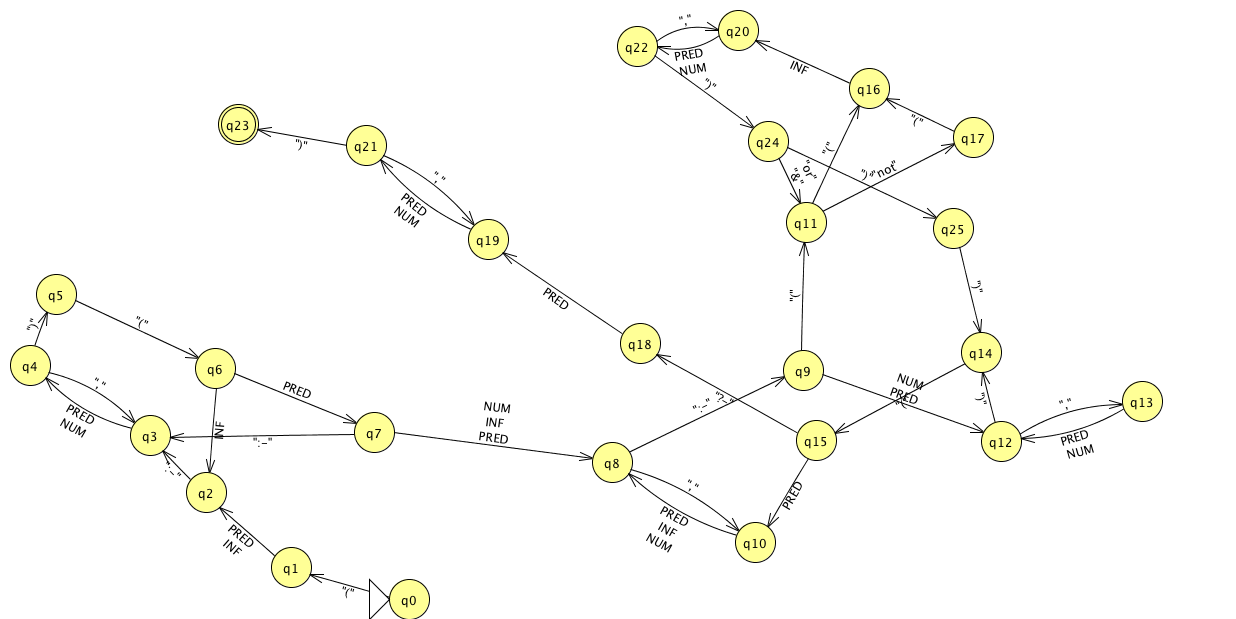
\includegraphics[width=1.3\textwidth,angle=90]{../images/PROGRAM.png}  
\caption{Autômato PROGRAM}
\end{figure}

\end{document} 

